\documentclass{beamer}
\usepackage[utf8]{inputenc}
\usepackage{hyperref}
\usepackage{colortbl}
\usepackage{epstopdf}
\usepackage{graphicx}
\usepackage{mathtools}
\usepackage{listings}
\usepackage{letltxmacro}
\usepackage{algorithm, algpseudocode}
\usepackage{listingsutf8}

\renewcommand{\lstlistingname}{Listing}
\interfootnotelinepenalty=10000
\lstset{
    %numbers=left,
    numberblanklines=false,
    captionpos=b,
    breaklines=true,
    frameshape={RYRYN}{ny}{yn}{RYRYN},
    literate={~} {$\sim$}{1}
}

\usepackage{pgfpages}
\setbeameroption{show notes on second screen=right}

\usetheme{Madrid}
\usecolortheme{seagull}
\title[\fontsize{0.08cm}{1em}\selectfont AHTN para Jogos em Tempo Real]{Adversarial Hierarchical-Task Network para Jogos em Tempo Real}
\author[Matheus de Souza Redecker]{Matheus de Souza Redecker
\\{\footnotesize Orientador: Prof. Dr. Felipe R. Meneguzzi}
}
\institute[PUCRS]{Pontifícia Universidade Católica do Rio Grande do Sul
\medskip\\
\url{matheus.redecker@acad.pucrs.br}
}
\date{30 de Novembro, 2016}
\begin{document}

%---------------------------------------------------------------------------------

    \begin{frame}
        \titlepage
    \end{frame}

%---------------------------------------------------------------------------------
%	{
%	\setbeamercolor{background canvas}{bg=lightgray}
%    \begin{frame}{Outline}
%       	\begin{itemize}
%       		\item \textbf{Introduction and Motivation}
%       		\item \textbf{Background}
%       		\item \textbf{Extracting Recognition Information From Domain Analysis}
%			\item \textbf{Landmark-based Plan Recognition}
%			\item \textbf{Planning-based Plan Abandonment Detection}
%			\item \textbf{Experiments and Evaluation}
%			\item \textbf{Related Work}
%			\item \textbf{Conclusion}			
%        \end{itemize}
%    \end{frame}
%	}
%---------------------------------------------------------------------------------

%Motivação

\begin{frame}{Motivação}
	\begin{itemize}
	    \item Inteligência Artificial em Jogos
	    \item Jogos de estratégia em tempo real
	    \item Algoritmo de Adversarial Hierarchical-Task Network
    \end{itemize}
    \note{
    	{\footnotesize
    	A IA em jogos faz com que os computadores sejam capazes de jogar sem intervenção humana. 
    	As técnicas são usadas para ter uma melhor interação com o usuario, e ele não perceber que está jogando contra uma maquina 
    	Mas as vezes as técnicas utilizadas nos jogos não são interamente de IA, pois elas podem utilizam conhecimentos proveniente do controle do jogo para tomar suas decisões. 
    	
    	Muitas vezes não há um tempo grande para decidir qual o proximo passo a ser tomado, com isso técnicas que tentam explorar todas as possibilidaes de um jogo se tornam ineficazes.
    	O Xadrez por exemplo tem $10^40$ estados possíveis do jogo é preciso algoritmos eficientes para gerar uma ação de forma rapida.
    	
    	O algoritmo de AHTN foi proposto para mitigar as limitações computacionais de abordagens tradicionais de raciocionio em jogos.
    	O algoritmo foi proposto por Santiago Ortanon  e combina técnicas de planejamento e busca adversária.
   	
    	 O intuito deste trabalho é explorar eficientemente o espaço de ações disponíveis no MicroRTS utilizando conhecimento de domínio, a fim de definir qual a próxima ação que deve ser executada.
	    }
    }
\end{frame}

    	
%O MicroRTS é uma simplificação de jogos como Stracraft e Age of Empires.
%Ele é um jogo RTS e foi desenvolvido em Java, para facilitar a codificação de técnicas de IA e servir de prova de conceito para as técnicas criadas
%Background
{
	\setbeamercolor{background canvas}{bg=lightgray}
	\begin{frame}{Background}
		\vspace{5mm}
		\begin{itemize}
			\item \textbf{Agentes}
			\item \textbf{Busca}
			\begin{itemize}
				\item \textbf{Busca adversária}
				\item \textbf{Minimax}
			\end{itemize}
			\item \textbf{Planejamento}       		
			\begin{itemize}
				\item \textbf{Planejamento Hierárquico}
				\item \textbf{AHTN}
			\end{itemize}
		\end{itemize}
	\end{frame}
}
%Agentes
\begin{frame}{Agentes}
	\begin{itemize}
		\item Ambiente
		\item Percepções
		\item Sensores
		\item Atuadores
		\item Ação
	\end{itemize}
	\begin{figure}[here]
		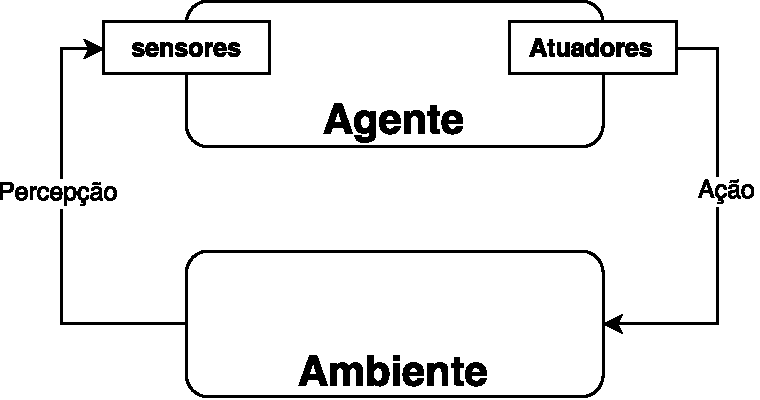
\includegraphics[width=0.45\linewidth]{fig/agente.pdf}	
	\end{figure}
	\note{
		agentes são entidades que agem de forma continua e autônoma em um ambiente, sendo capazes de receber estímulos do ambiente através de sensores, e assim responder aos estímulos por intermédio de atuadores. Para os agentes os estímulos do ambiente são recebidos como percepções. Os atuadores por sua vez, geram uma ação considerando as percepções 	
	}
\end{frame}
%BUSCA
\begin{frame}{Busca}
\begin{itemize}
	\item Ações
	\item Função de transição
	\item Objetivo
\end{itemize}

\begin{figure}[here]
	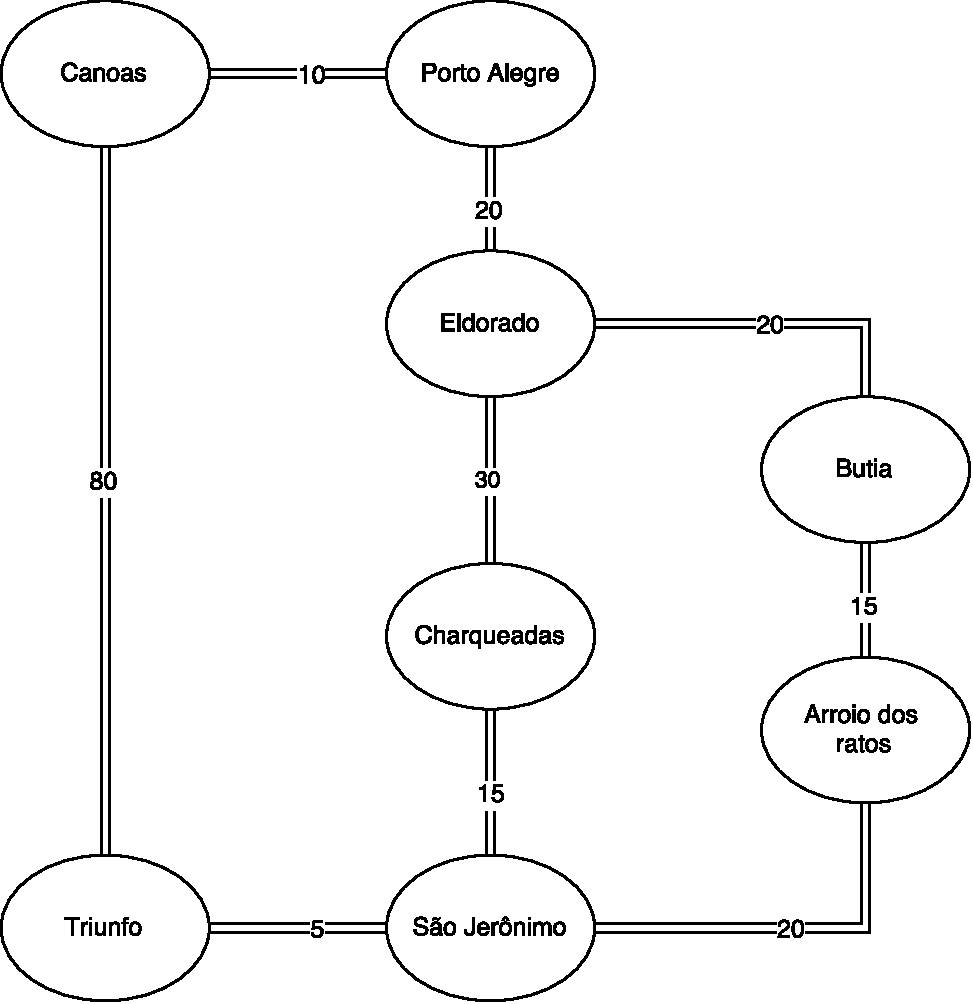
\includegraphics[width=0.3\linewidth]{fig/mapabusca.pdf}
\end{figure}
\note{
	Técnicas de busca tem como objetivo encontrar uma sequência de ações para que um agente alcance um determinado objetivo.\\	
	As ações são executadas por agentes no ambiente\\	
	A função de transição define que quando um agente está em um estado e executa determinada ação ele vai para outro estado\\
	O objetivo do agente é alcançar alguma coisa	
	}
\end{frame}
\begin{frame}{Busca adversária}
	\begin{itemize}
		\item Árvore das jogadas (\textit{game tree})
		\item Estado terminal
		\item Utilidade
	\end{itemize}
	
	\begin{figure}[here]
		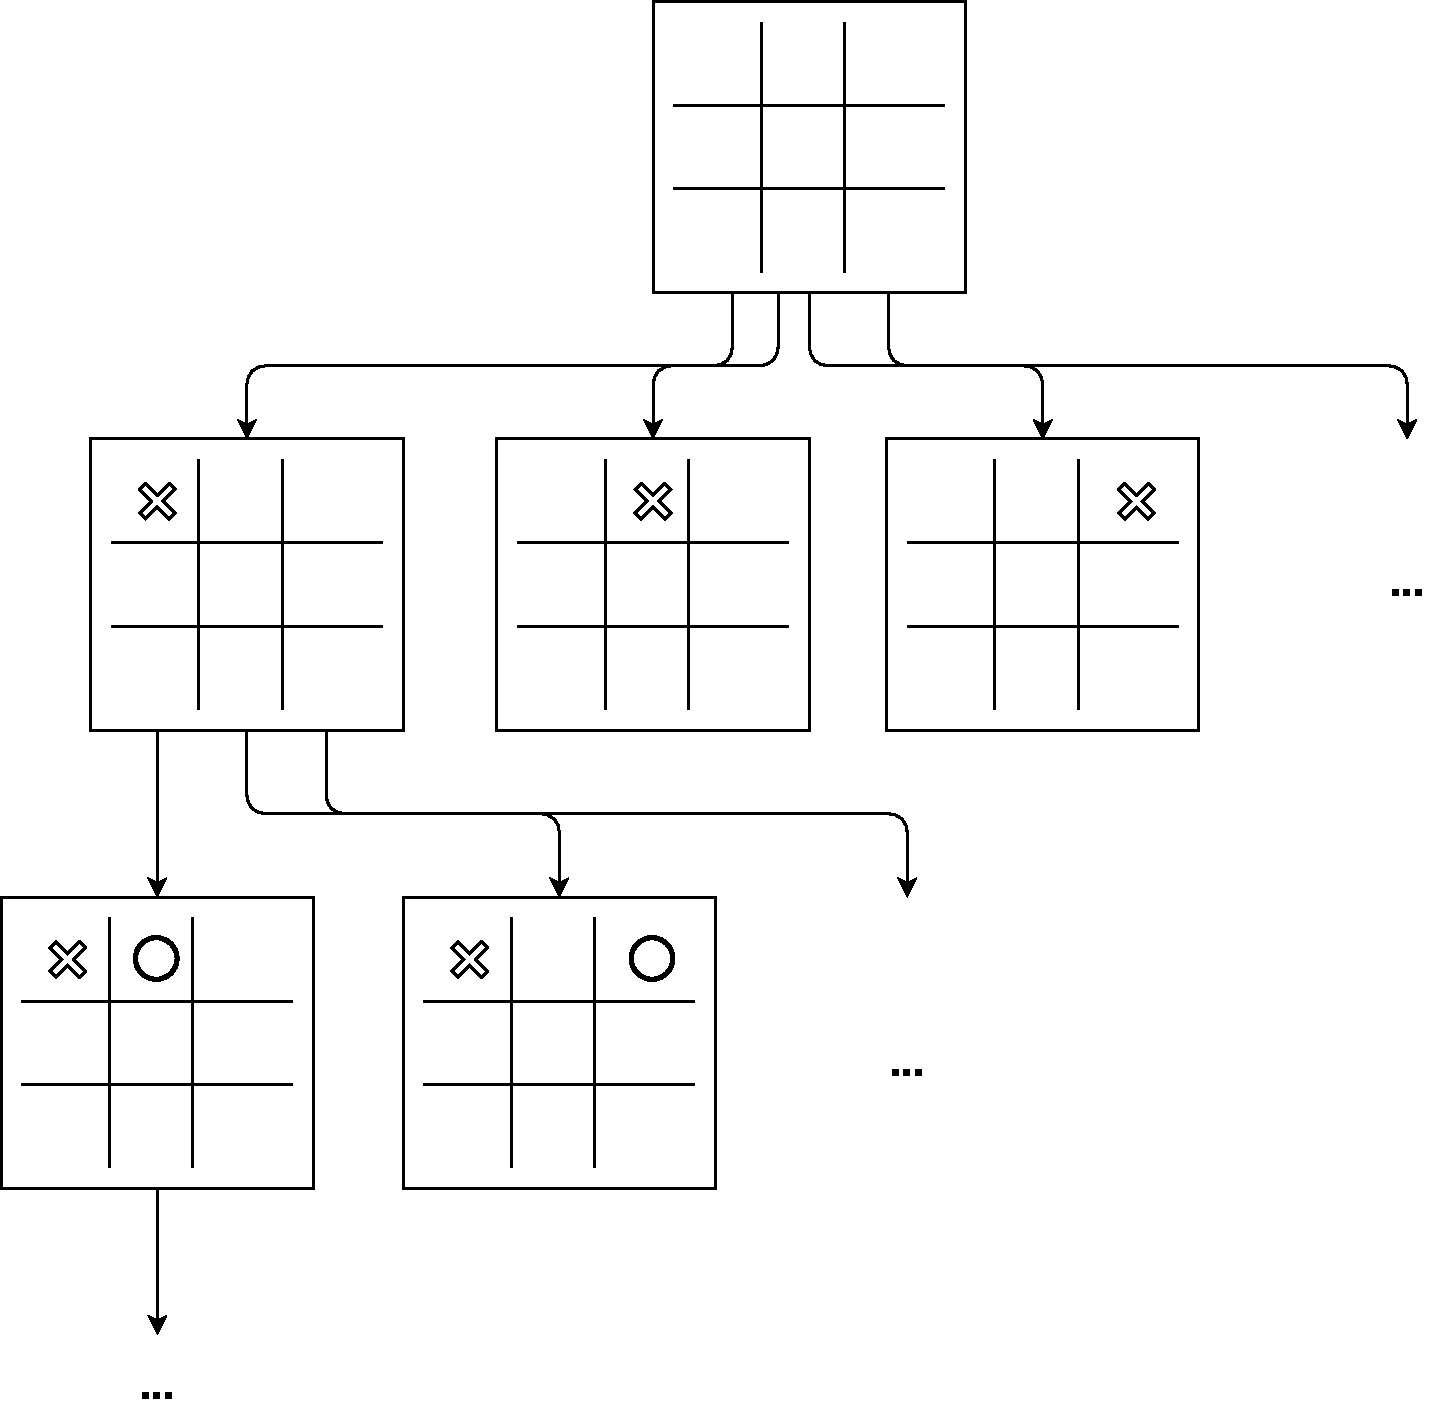
\includegraphics[width=0.45\linewidth]{fig/jogodavelha.pdf}	
	\end{figure}
	\note{
		Já a busca adversária é utiliza em ambientes competitivas que possuam mais de um agente \\
		As técnicas utilizam a arvore das jogadas para percorrer o espaço de estados dos jogos\\
		Por exemplo, no jogo da velha, cada possibilidade de jogada deve ser percorrida para que o algoritmo possa determinar qual a melhor jogada\\
		O estado terminal indica quando o jogo chegou ao fim\\
		Cada estado do jogo pode ter um valor de utilidade, que é obtido através de uma função de avaliação\\
		A função de avaliação pode utilizar uma heuristica para determinar o estado do ambiente\\
		Esse valor serve para determinar o quão bom é o estado, ou ruim
	}
\end{frame}

%Minimax
\begin{frame}{Minimax}
	\vspace{-3mm}
	\begin{figure}[here]
		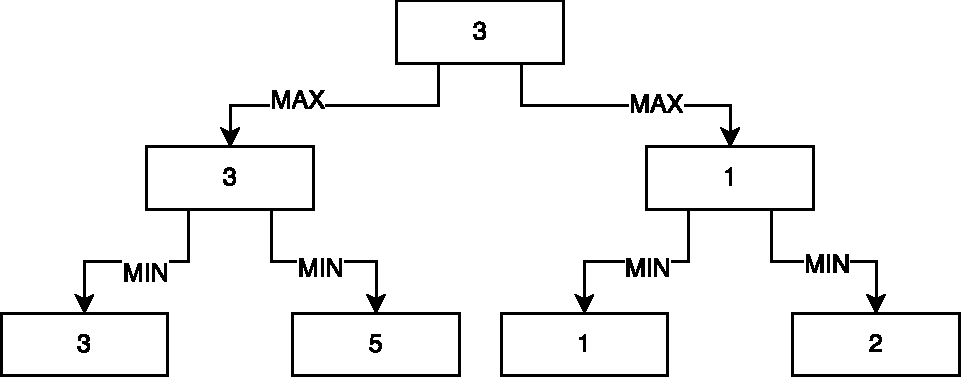
\includegraphics[width=0.8\linewidth]{fig/gametree.pdf}	
	\end{figure}	
	\note{
		O algoritmo de Minimax é um algoritmo de busca adversária que tem como objetivo determinar qual a melhor jogada para o estado atual. \\
		Este método considera dois agentes que estão competindo entre si\\
		O agente Max representa a perspectiva que está tentando aumentar as recompensas das suas ações.\\
		Já o agente Min é com quem o Max está jogando contra, e suas ações estão tentando ser minimizadas.\\
		Por exemplo, quando Min tem duas possibilidades de jogadas, uma boa e uma ruim, o algoritmo seleciona a ruim como melhor opção para Max, pois quanto menor a chance de Min ter uma jogada de sucesso, melhor para ele.
	}
\end{frame}

%Planejamento
\begin{frame}{Planejamento}
	
	\vspace{-3mm}
	\begin{figure}[here]
		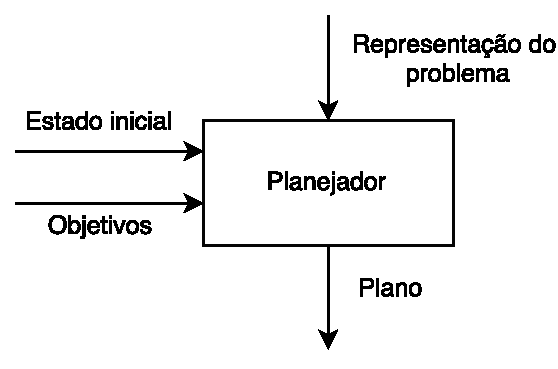
\includegraphics[width=0.6\linewidth]{fig/modelo.pdf}	
	\end{figure}	
	\note{
		Planejamento estuda o processo de geração de planos de forma computacional. \\
		O planejador utiliza uma representação do domínio, que contém informações das ações disponíveis no ambiente. E apartir de um estado inicial, e um objetivo que o agente deseja alcançar, o planejador encontra a sequencia de ações que parte do estado inicial e alcança seus objetivos. 	
	}
\end{frame}
%Planejamento Hierárquico
\begin{frame}{Planejamento Hierárquico (HTN)}
	\begin{itemize}
		\item Tarefas alto nível
		\item Conhecimento de domínio
		\item Decomposições
		\item Tarefas primitivas
	\end{itemize}
	\vspace{-3mm}
	\begin{figure}[here]
		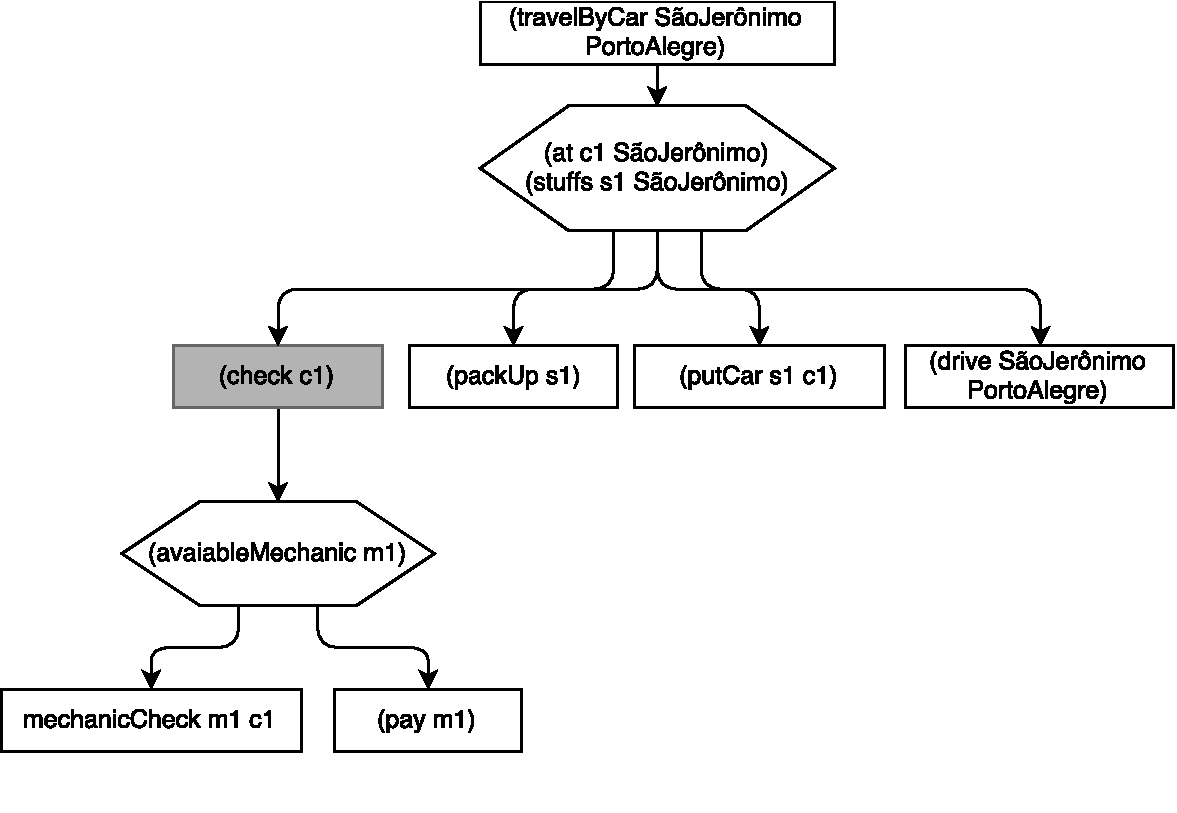
\includegraphics[width=0.7\linewidth]{fig/htnmethodresult.pdf}	
	\end{figure}	
	\note{
		Problemas de grande complexidade acabam demorando muito com planejamento clássico. \\
		Como alternativa para isso, foi proposto o planejamento hierarquico, ou HTN. \\
		Ele se diferencia do anterior pelo fato de que as tarefas são tratadas em mais alto nivel, ou seja, as tarefas em alto nível, chamadas de tarefas não primitivas, são decompostas em tarefas menores, chamadas de primitivas, e assim por diante até que restem tarefas primitivas, que possam ser realizadas no ambiente. \\
		Para isso, é preciso um conhecimento de domínio que contém informações relativas as ações disponíveis e transições que são feitas no ambiente. \\
		Por exemplo, para realizar uma viajem de carro, não é só pegar o carro e dirigir, é preciso ir ao mecânico, fazer as malas, colocar as malas no carro, e então viajar.
		
		As tarefas primitivas são as tarefas que fazem parte do plano!
	}
\end{frame}

%Algoritmo de AHTN
\begin{frame}{Adversarial Hierarchical-Task Network}
	\begin{itemize}
		\item Como funciona o algoritmo?
		\item Minimax + planejamento hierárquico
	\end{itemize}
	
	\begin{figure}[here]
		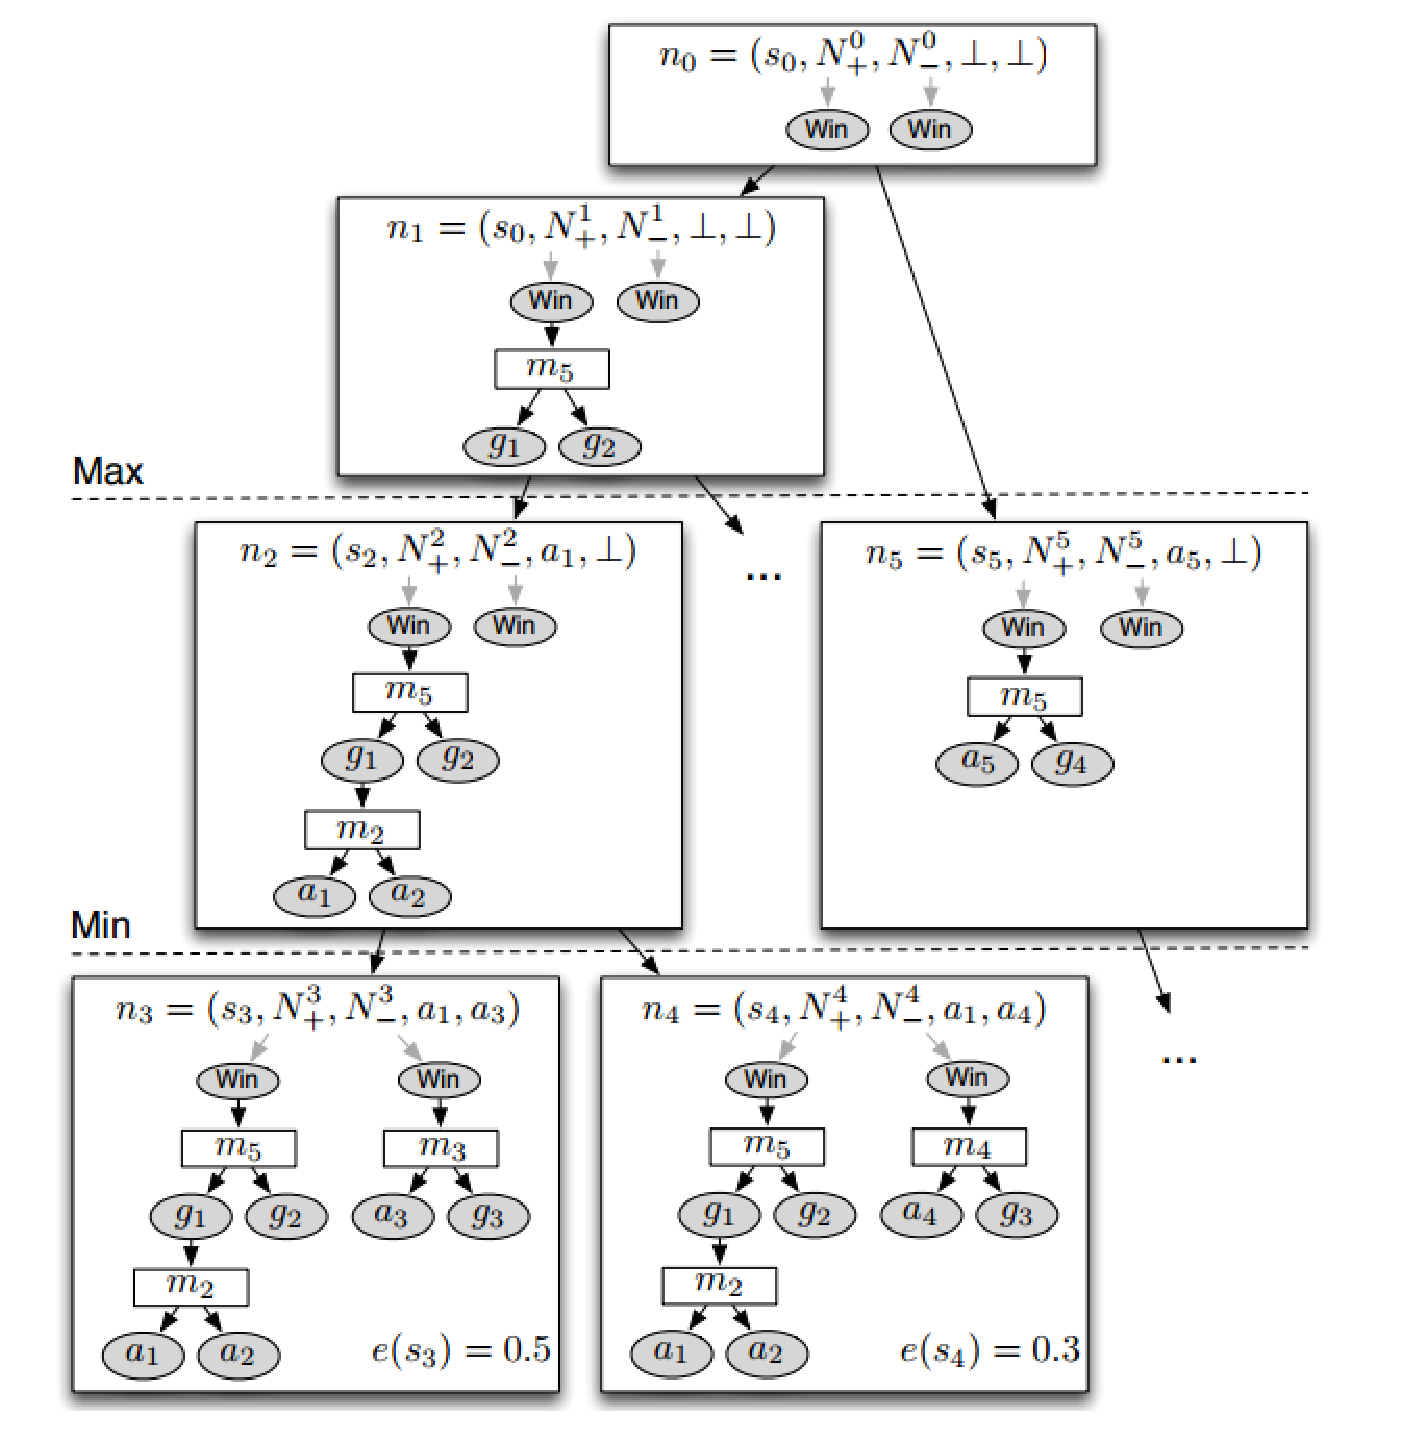
\includegraphics[width=0.4\linewidth]{fig/ahtn.pdf}	
	\end{figure}	
	
	\note{
		O algoritmo de AHTN é uma combinação do algoritmo de Minimax com o conhecimento de domínio do planejamento hierarquico \\
		O algoritmo visa encontrar os melhores planos para Min e para Max \\
		Para isso, os planos de cada um das perspectivas vão sendo decompostos. \\
		O algoritmo pode ir até uma determinada profundidade, ou decompor todo os espaço de estados \\
		A grande diferença do algoritmo é que a troca de perspectivas é feita apenas quando há uma tarefa primitiva a ser realizada no ambiente, caso o contrario o algoritmo decompõe as tarefas não primitivas e segue na mesma perspectiva
	}
\end{frame}


%MicroRTS+JSHOP2
{
	\setbeamercolor{background canvas}{bg=lightgray}
	\begin{frame}{Recursos Utilizados}
		\vspace{5mm}
		\begin{itemize}
			\item \textbf{MicroRTS}
			\item \textbf{JSHOP2}
		\end{itemize}
	\end{frame}
}
%MicroRTS
\begin{frame}{MicroRTS}
	\begin{itemize}
		\item O que é?
		\item Construções
		\item Unidades
		\item Técnicas
		\item Camada de abstração
	\end{itemize}
	\vspace{-3mm}
	\begin{figure}[here]
		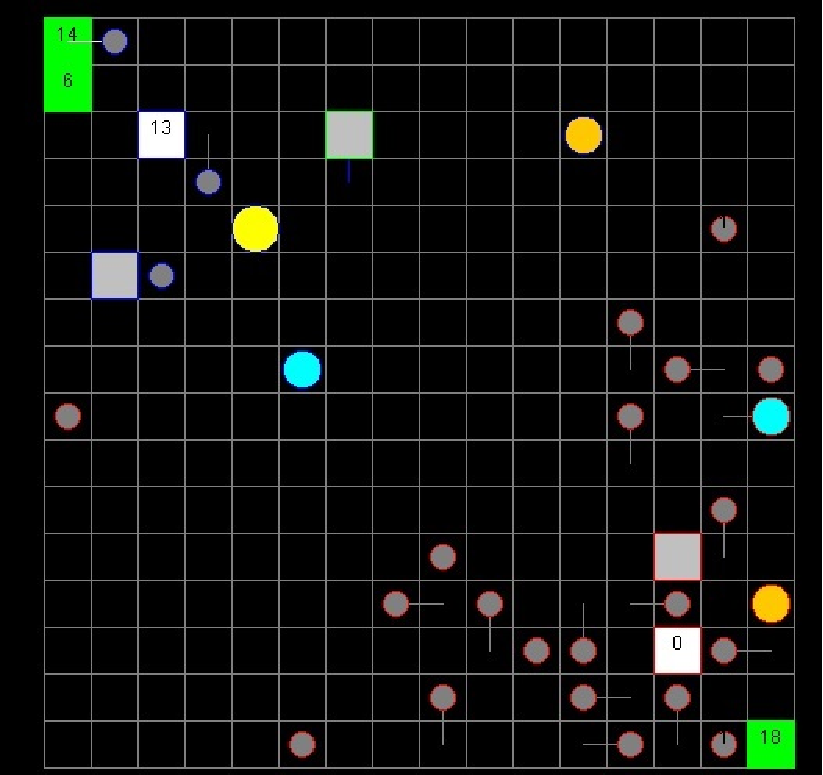
\includegraphics[width=0.4\linewidth]{fig/microrts.pdf}	
	\end{figure}	
	\note{
		O MicroRTS é um jogo de estrategia em tempo real, criado por Santiago Ortanon em java \\
		É um framework que permite a implementação de técnicas de IA \\
		Construções: base - edificação prinicipal, e quartel- treinar unidades de ataque \\
		Unidades: 3 unidades de ataque, 1 ataca de longe, 1 forte, 1 rapida e fraca \\
		Técnicas: comportamentos pre determinados (script), MonteCarlo, Minimax, Portifolio Search 
		
		Camada de abstração- fornece as ações do jogos em classes para serem executadas\\
		Toda IA precisa do método getaction para retornar a ação
	}
\end{frame}
%JSHOP2
\begin{frame}{JSHOP2}
	\begin{itemize}
		\item Planejador
		\item Domínio
		\item Problema
	\end{itemize}	
	\note{
		O JSHOP2 é um sistema de planejamento independente de domínio baseado em HTN. \\
		O JSHOP2 foi desenvolvido em Java por Dana Nau e sua equipe de pesquisa.
		
		O JSHOP2 preciso de 2 arquivos de entrada para gerar o plano\\
		O domínio contém as descrições dos operadores (tarefas primitivas), e dos métodos (tarefas não primitivas) \\
		O problema contém a especificação do estado inicial do ambiente, junto com uma ou mais tarefas que desejam ser executada
		
		O JSHOP2 gera as tarefas primitivas do plano\\
		O JSHOP2 foi escolhido por ser em java
	}
\end{frame}

{
	\setbeamercolor{background canvas}{bg=lightgray}
	\begin{frame}{Implementação}
		\vspace{5mm}
		\begin{itemize}
			\item \textbf{Ações do MicroRTS}
			\item \textbf{Modelagem do domínio}
			\item \textbf{Heurísticas}
			\item \textbf{Geração dos Planos}
			\item \textbf{Algoritmo AHTN}
		\end{itemize}
	\end{frame}
}

%Ações
\begin{frame}{Ações do MicroRTS}

	\begin{figure}[here]
		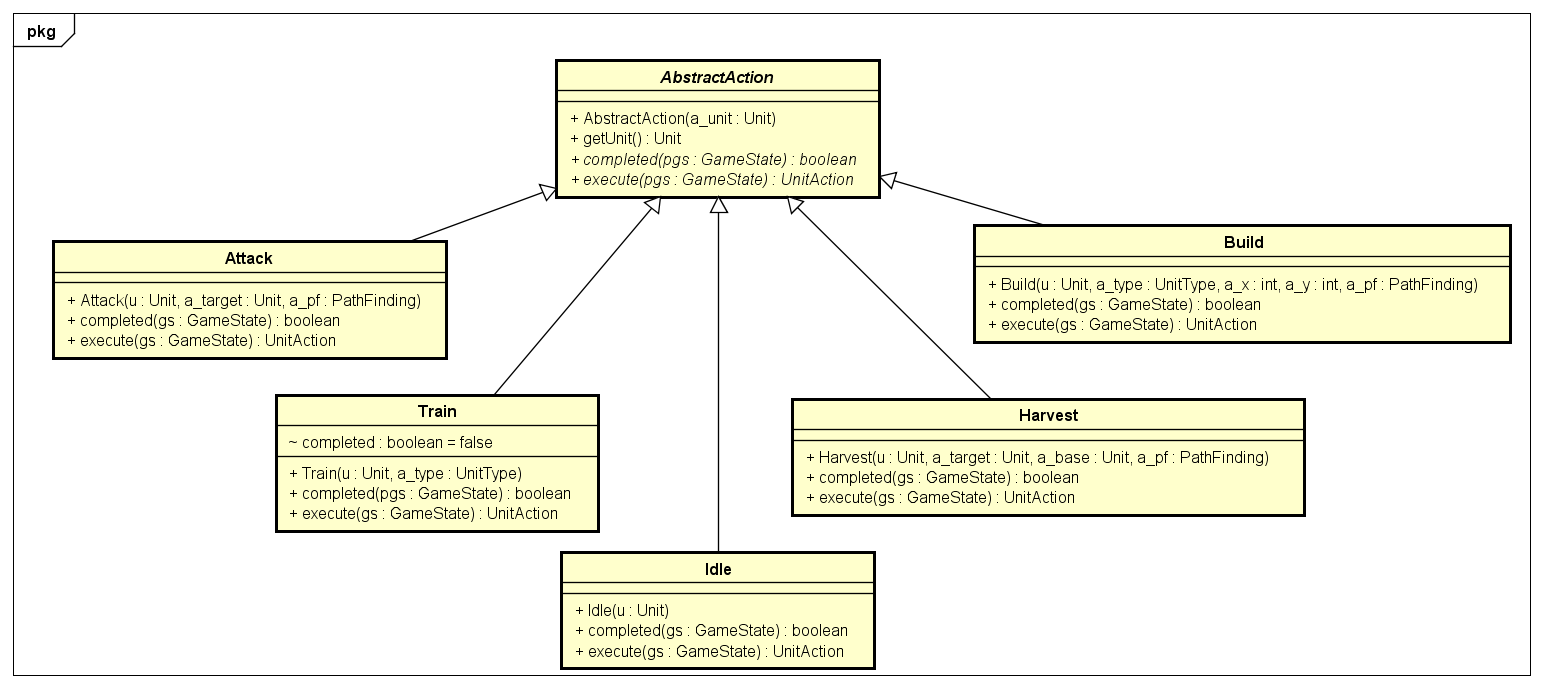
\includegraphics[width=1\linewidth]{fig/acoesmicro.png}	
	\end{figure}
	\note{
		A camada de abstração fornece essas classes \\
		Mas ainda assim, é preciso dizer qual unidade realiza cada método \\
		Para isso, para cada ação disponível na camada, foi feita um método em Java relativo \\
		Por exemplo, somente o worker pode extrair recurso, para isso é preciso saber qual recurso vai ser extraído e em qual base o recurso será armazenado
	}
\end{frame}
%Modelagem do Domínio
\begin{frame}{Modelagem do Domínio}
	\begin{itemize}		
		\item Operadores
		\item Métodos
		\item Unidade de ataque
	\end{itemize}
	\note{
		Foram criados dois domínios \\
		A grande diferença dos domínio é que no primeiro domínio, apenas uma unidade de ataque é criada \\
		Já no segundo domínio, podem haver mais de uma unidade \\
		
		Nos dois domínios, apenas uma base, um trabalhador e um quartel são criados\\ 
		O trabalhador fica responsável por extrair recursos e construir as edificações quando necessario \\
		O quartel cria as unidades de ataque \\
		
		Os operadores do domínio, são as operações que podem ser executados no MicroRTS \\
		Já os métodos implementam as regras do jogo \\
		Como por exemplo, apenas um quartel pode ser criado, então o método deve garantir que apenas quando não houver quartel que o método é chamado.
	}
\end{frame}
%Heurística
\begin{frame}{Heurísticas}
	\begin{itemize}
		\item Unidades adversárias
		\item Pesos
		\item Estado terminal
	\end{itemize}
	\vspace{5mm}
	\begin{equation}
		h1 =  (1*worker) + (5 * quartel) + (10 * base) + (2 * unidadesDeAtaque)
	\end{equation}
	
	\begin{equation}
		h2 =  h1(jogador) - h1(inimigo)
	\end{equation}
	\note{
		Foram criados duas heuristicas \\
		A heuristica 1 é feita para levando em conta as unidades que o jogador possui. \\
		Os pesos são relativos a quanto custa de recursos para cada unidade ser construida\\
		Mas assim, as unidades do inimigo não são levadas em consideração,
		Um inimigo pode ter varias unidades contra uma do jogador, isso faz com que ele esteja perdendo\\
		Para contornar esse problema, foi criado a heuristica 2, nela o valor obtido da heuristica 1 para o jogador é diminuido do valor obtido para as unidades inimigas.
		
		A heuristica indica um estado terminal para um dos jogadores em 2 determinadas situações do jogo: \\
		Só existe uma base e não há recursos para fazer worker\\
		Só existe worker e não há recursos para fazer base 
	}
\end{frame}
%Geração dos Planos
\begin{frame}{Geração dos Planos}
	\begin{figure}[here]
		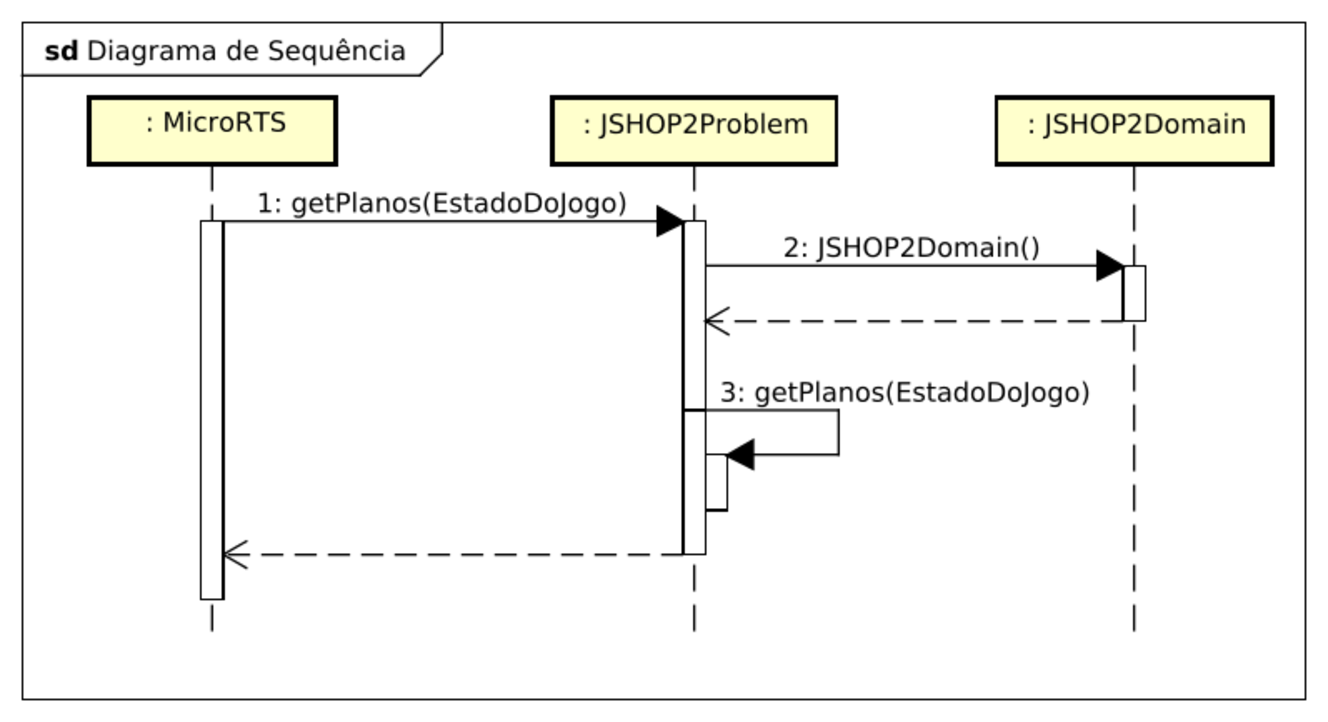
\includegraphics[width=0.9\linewidth]{fig/gerarPlano.pdf}	
	\end{figure}	
	\note{
		O JSHOP2 gera duas classes java, uma relativa ao domínio e uma relativo ao problema\\
		Essas classes traduzem as informações do domínio e do problema para estruturas java \\
		
		Como o domínio é estatico e não é alterada em nenhuma execução\\
		Já o problema muda a cada nova configuração do ambiente\\
		Para conseguir gerar os planos dentro do MicroRTS foi preciso criar uma classe java que representasse o Estado do Jogo\\
		Nela está contido as informações provenientes do jogo, e então é possível converter as informações para as estruturas utilizadas pela classe java do JSHOP2
		
		Assim o MicroRTS chama a geração dos planos, a classe do problema instancia um domínio, e então com as informações do jogo os planos são gerados
	}
\end{frame}
%Implementação
\begin{frame}{Algoritmo de AHTN}
	\begin{itemize}
		\item Diferenças
		\item Tempo das ações
	\end{itemize}
	\note{
		O JSHOP2 gera apenas as tarefas primitivas que devem ser executados para alcançar o plano \\
		Por essa razão, o algoritmo passou por uma adaptação\\
		A cada chamada há uma troca de perspectiva \\
		Pelo fato de que não há a informação com o JSHOP2 dos métodos que estão sendo usados para a decomposição das tarefas
		
		As tarefas dentro do MicroRTS levam alguns ciclos para serem realizadas\\
		Por essa razão foi estipulado um valor de 50 rounds de jogo para que o algoritmo gere uma jogada novamente
	}
\end{frame}
\begin{frame}{Pseudo código do AHTN implementado}
	\vspace{5mm}
	{\footnotesize
		\begin{algorithmic}[1]		
			\Function {AHTNMax}{$estado, planoMax, planoMin, prof$}
			\If {$terminal(estado) \vee prof \leq 0$}
			\State	\Return $(planoMax, planoMin, avaliacao(estado))$
			\EndIf
			\State {$nextAction(planoMax)$}
			\State $(Pmax', Pmin', ev') = \perp, \perp, -\infty$
			\ForAll{$plano \in getPlanos(estado)$}
			\State $(Pmax, Pmin, ev) = \Call{AHTNMin}{(estado, planoMax, planoMin, prof-1)}$
			\If {$ev' > ev$}
			\State $(Pmax', Pmin', ev') = (Pmax, Pmin, ev)$
			\EndIf		 		 		
			\EndFor
			\State \Return $(Pmax', Pmin', ev')$
			\EndFunction
		\end{algorithmic}	
	}
	\note{
		O algoritmo começa testando se a profundidade chegou ao fim ou se o estado é terminal
		Caso isso não acontece, uma ação é executada do plano, e então para cada ação possível nesse novo estado do jogo para Min é gerado os planos, assim o algoritmo seleciona o plano com a maior função de avaliação.
		
		O algoritmo AHTNMin é analogo, mas ao inves da maior função de avaliação é buscado a menor
	}
\end{frame}

%Resultados
{
	\setbeamercolor{background canvas}{bg=lightgray}
	\begin{frame}{Resultados}
		\vspace{5mm}
		\begin{itemize}
			\item \textbf{Mapas}
			\item \textbf{Tamanho das técnicas}
			\item \textbf{Tempo de geração das ações}
		\end{itemize}
	\end{frame}
}
\begin{frame}{Mapas}
	\begin{itemize}
		\item Mapa 1
		\begin{itemize}
			\item 16x16, base e trabalhador
			\item Domínio HTN 2
		\end{itemize}
		\item Mapa 2
		\begin{itemize}
			\item 8x8, base, trabalhador e quartel
		\end{itemize}
		\item Mapa 3
		\begin{itemize}
			\item 8x8, base, trabalhador e obstáculos
			\item Domínio HTN 2
		\end{itemize}
		\item Lado do jogo
	\end{itemize}
	
	\begin{figure}[here]
		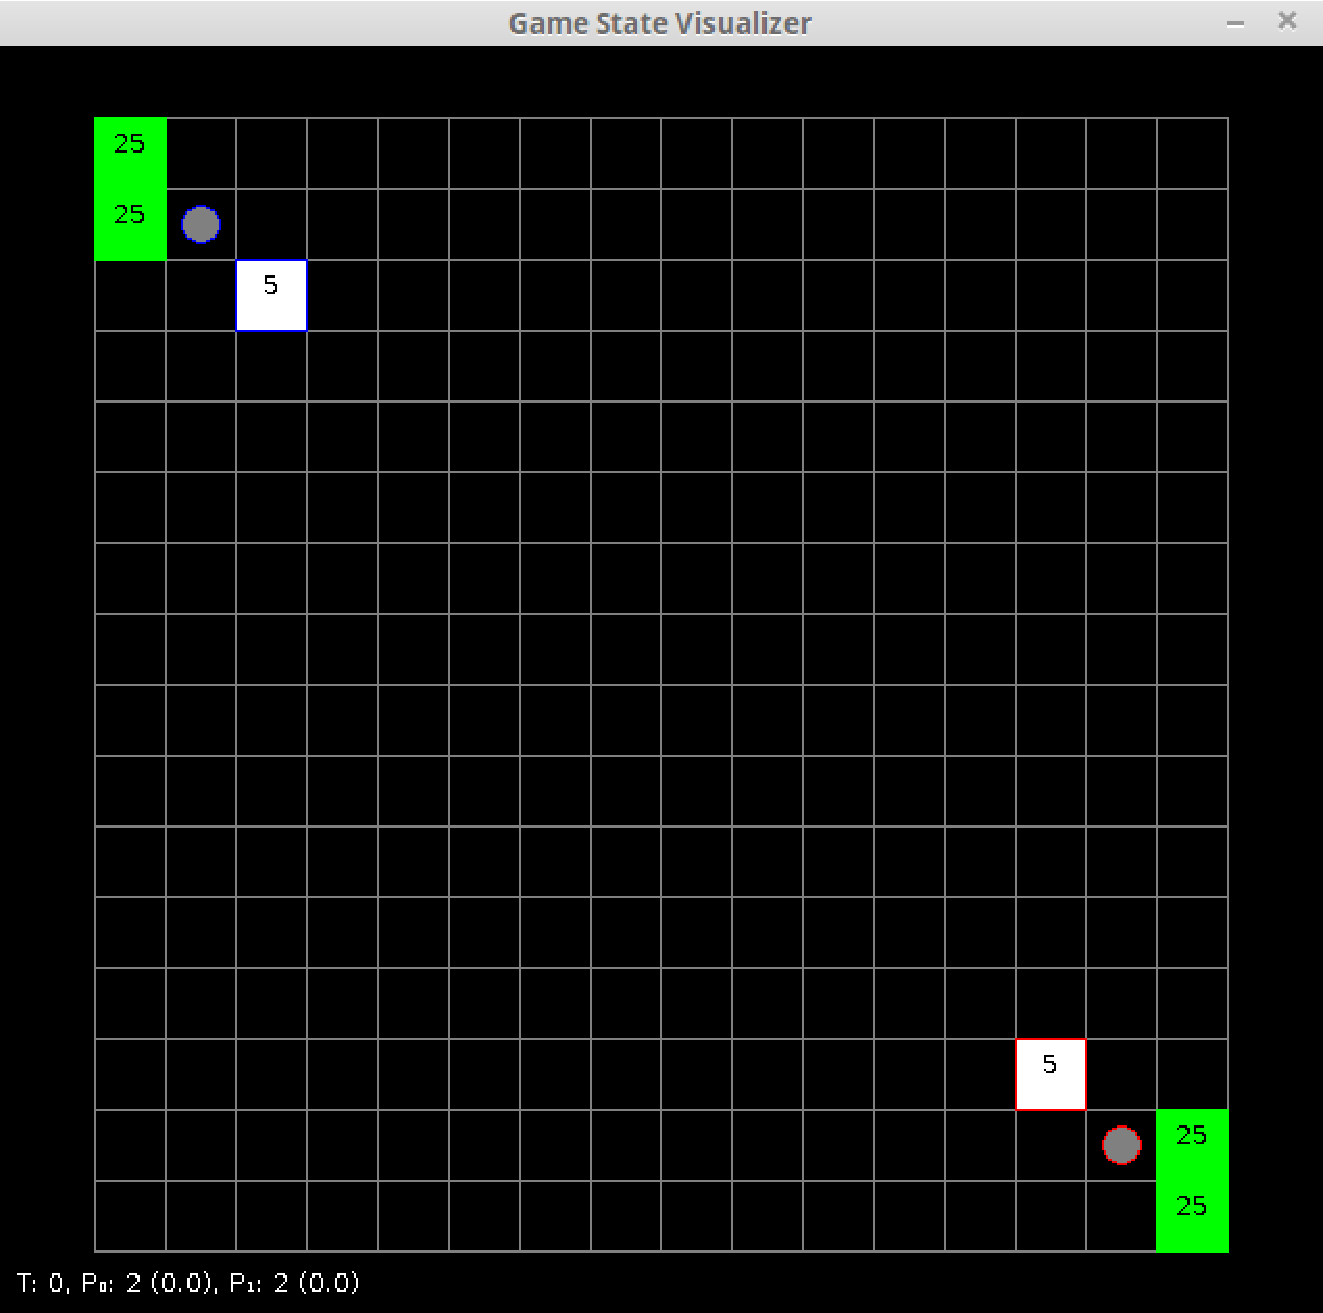
\includegraphics[width=0.25\linewidth]{fig/map16x16.pdf} \quad
		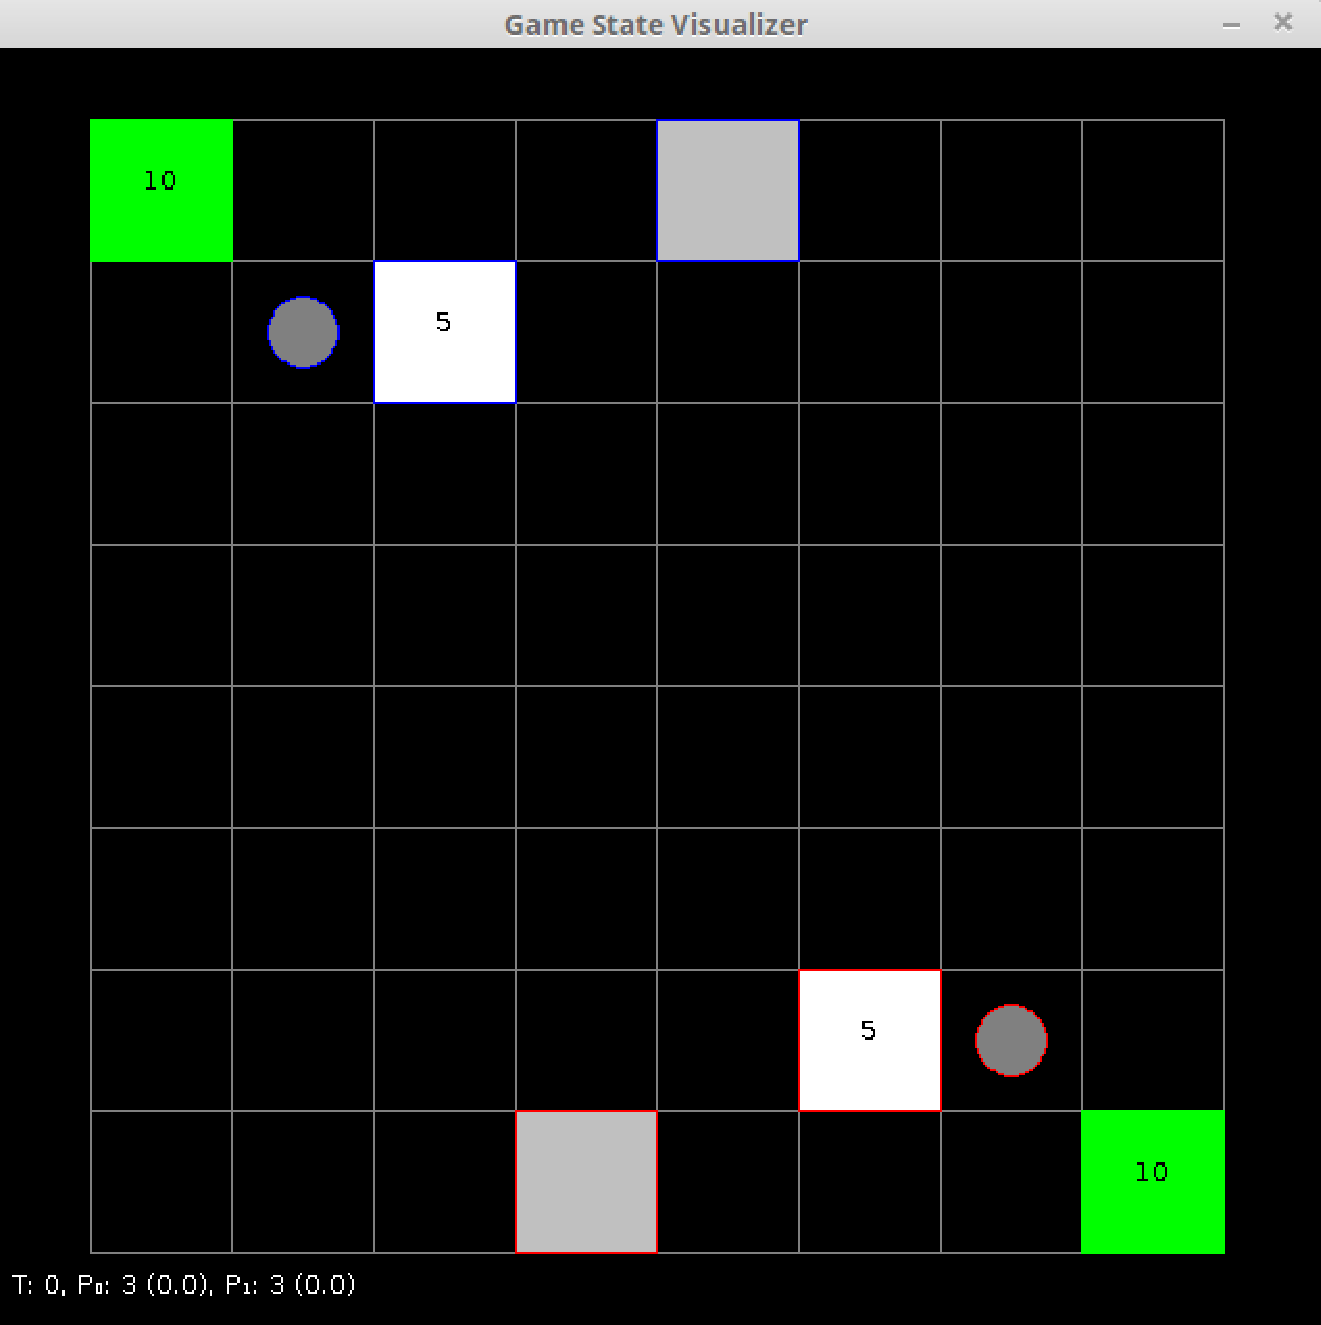
\includegraphics[width=0.25\linewidth]{fig/map8x8quartel.pdf} \quad
		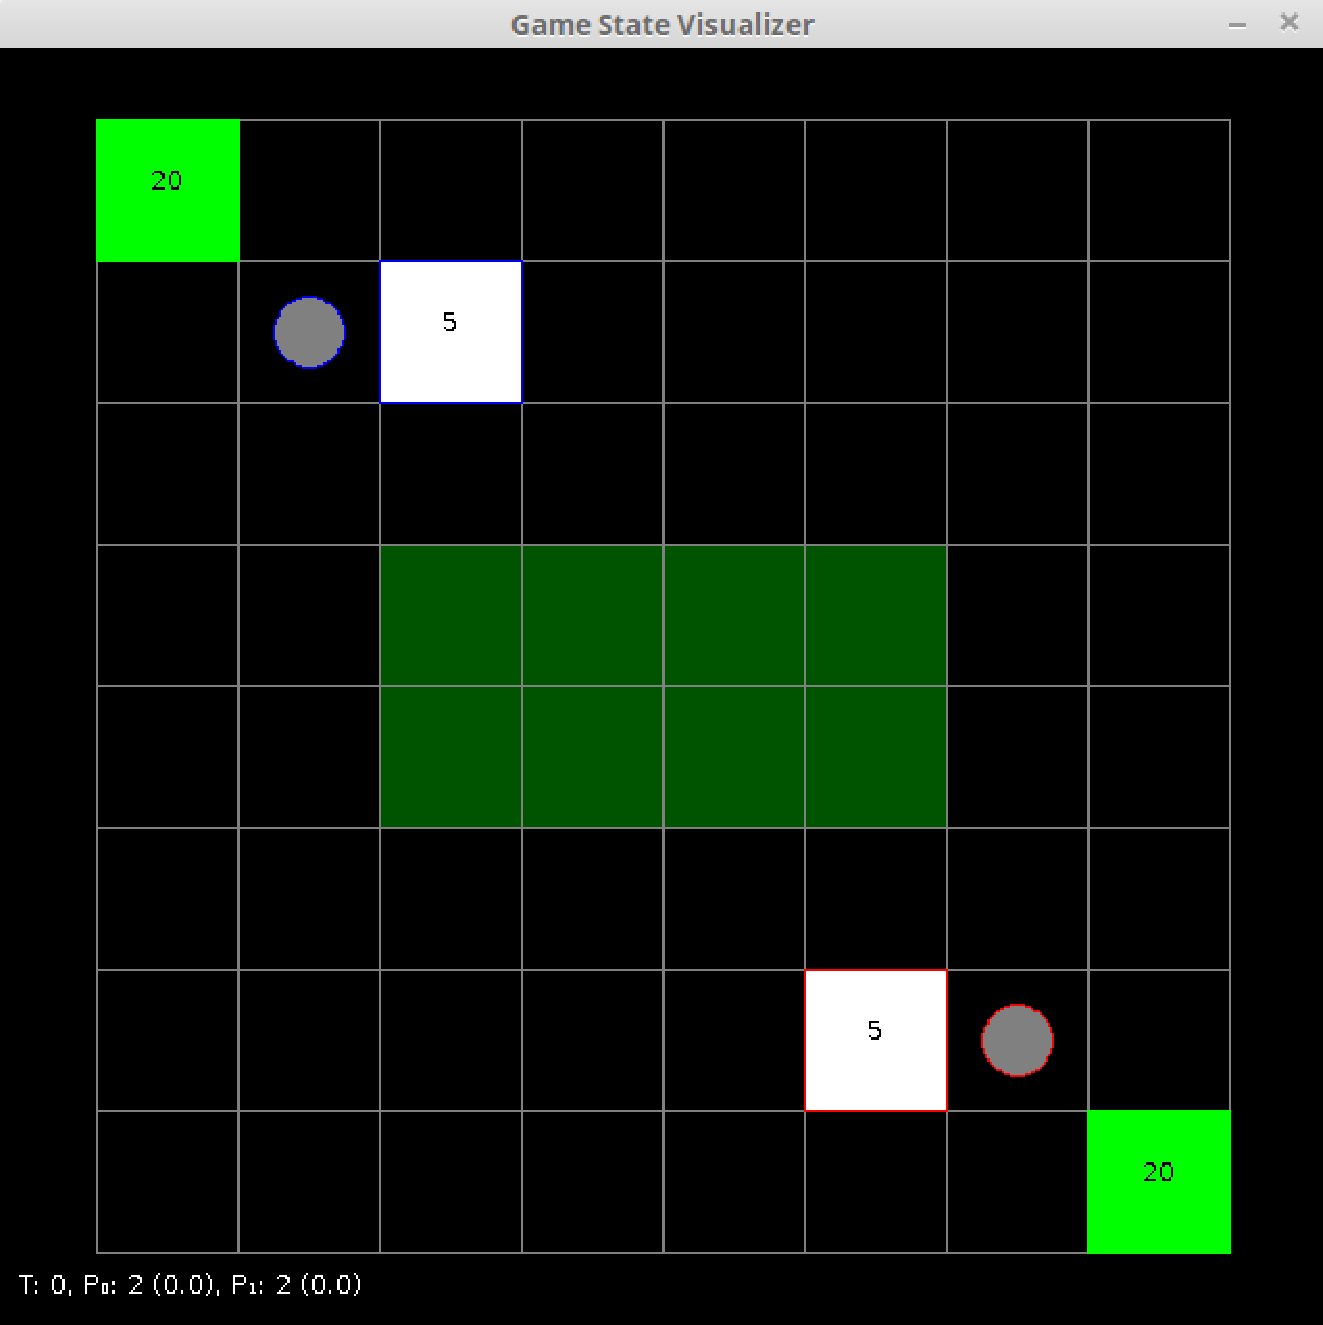
\includegraphics[width=0.25\linewidth]{fig/map8x8obsta.pdf} 
	\end{figure}
	\note{
		A avaliação dos resultados foi feita em três mapas e com 10 jogos 
		
		O mapa 1 e 3 apresentam melhor desempenho no domínio 2, pelo fato de que varias tropas são criadas e técnicas que não ganhavam passam a ganhar no outro domínio
		
		O mapa 2 perde rapido pois as técnicas são muito violentas
		
		O lado do jogo influencia muito nos resultados, pois no lado vermelho no mapa 1 é posicionado em melhor local para criação das tropas\\
		Nos demais mapas, as técnicas no MicroRTS não se comportam da mesma maneira que no outro lado\\
		Elas demoram um pouco para atacar e com isso dão tempo do AHTN criar tropas
	}
\end{frame}

%Tamanho da IA
\begin{frame}{Tamanho das técnicas}
	\begin{center}
		\begin{tabular}{|c|c|c|}
			\hline
			\textbf{Adversário} & \textbf{Tamanho} & Porcentagem de vitórias \\ \hline
			Domínio 1           & 19,9 kB          & -             \\ \hline
			Domínio 2           & 20,1 kB          & -           \\ \hline
			RandomBiasedIA      & 4,6 kB           & 80\%             \\ \hline
			WorkerRush          & 13,6 kB          & 0\%             \\ \hline
			MonteCarlo          & 18,1 kB          & 30\%             \\ \hline
		\end{tabular}
	\end{center}
	\note{
		Foi utilizado o algoritmo de compressão do zip para medir o tamanho de código das técnicas\\
		A maior técnica presente no MicroRTS é a MonteCarlo, o algoritmo ocnsegue ganhar 30\% dela.
		
		A técnica de WorkerRush não perdeu em nenhum teste, e ela apersente um tamanho mediano em relação as demais técnicas
		
		Uma das técnicas mais simples é a Random, e ela em alguns casos consegue vencer 
		
		Os domínios ficaram pesados pela integração do JSHOP2 na geração dos planos, por essa razão eles acabaram ficando com o maior peso entre as técnicas	
	}
\end{frame}
%Geração das ações
\begin{frame}{Tempo de geração das ações}
	\begin{figure}[here]
		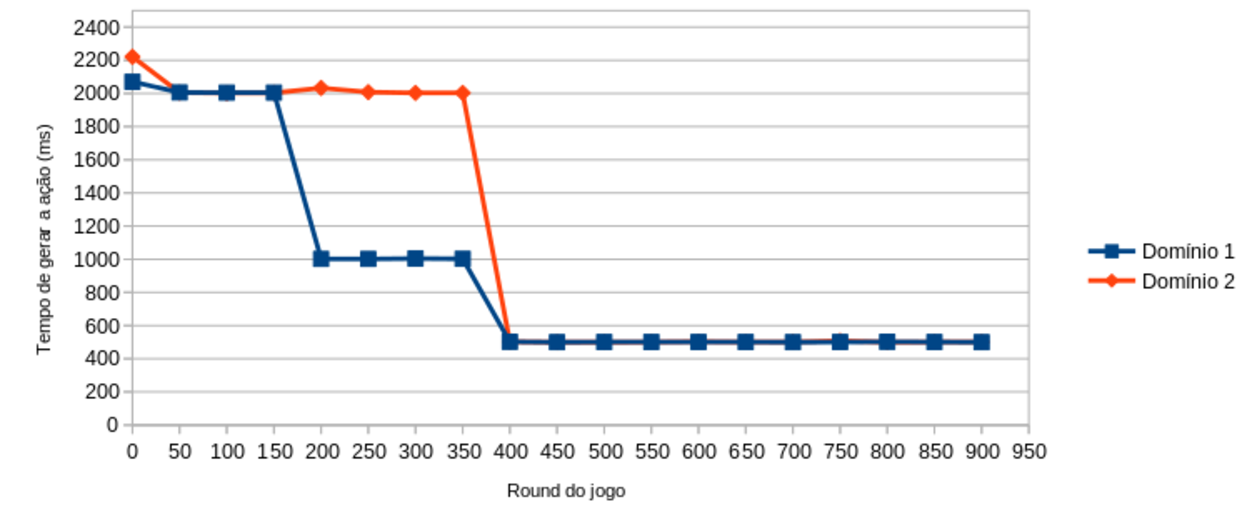
\includegraphics[width=0.9\linewidth]{fig/graph.pdf}
	\end{figure}
	\note{
		isso ocorre porque há menos ações que podem ser realizadas no jogo, o que implica em menos níveis na árvore de busca que o algoritmo tem que percorrer.\\
		No final do jogo, o jogador já tem tropas de ataque e apenas manda elas atacar.	
	}
\end{frame}

%Conclusao
\begin{frame}{Conclusão}
	\begin{itemize}
		\item Problemas
		\item Influência do domínio
		\item Trabalhos futuros
	\end{itemize}
	\note{
		O objetivo inicial era integar uma técnica de Machine Learning ao algoritmo para tentar melhorar os resultados\\
		Devido ao tempo perdido na integração do JSHOP2 com o MicroRTS e na criação do domínio, isso não foi possível
		
		O principal problema do algoritmo é no tempo de geração das ações, pois todas as outras técnicas do microRTS levam 1 milissegundo para gerar uma ação, enquanto o algoritmo leva no minimo meio segundo, isso prejudica o desempenho em jogos RTS 
		
		O domínio tem influencia nos resultados, pois como ele não possui um plano de contingencia, por exemplo, nas técnicas que criam trabalhadores para atacar, o domínio segue criando seu quartel para criar suas unidades de ataque, com isso ele acaba sendo destruido muito rapido, pois não há tempo de reagir.	
		
		Como trabalhos futuros- Acoplar uma técnica de Machine Learning - Implementar um mecanismo de tempo de procura por uma ação - Criar domínios mais abrangentes
	}
\end{frame}

	{
		\setbeamercolor{background canvas}{bg=lightgray}
		\begin{frame}{}
			\centering
			Obrigado!
		\end{frame}
	}  


\end{document}